
\section{Introduction}


\begin{figure}[!t]
  \centering
  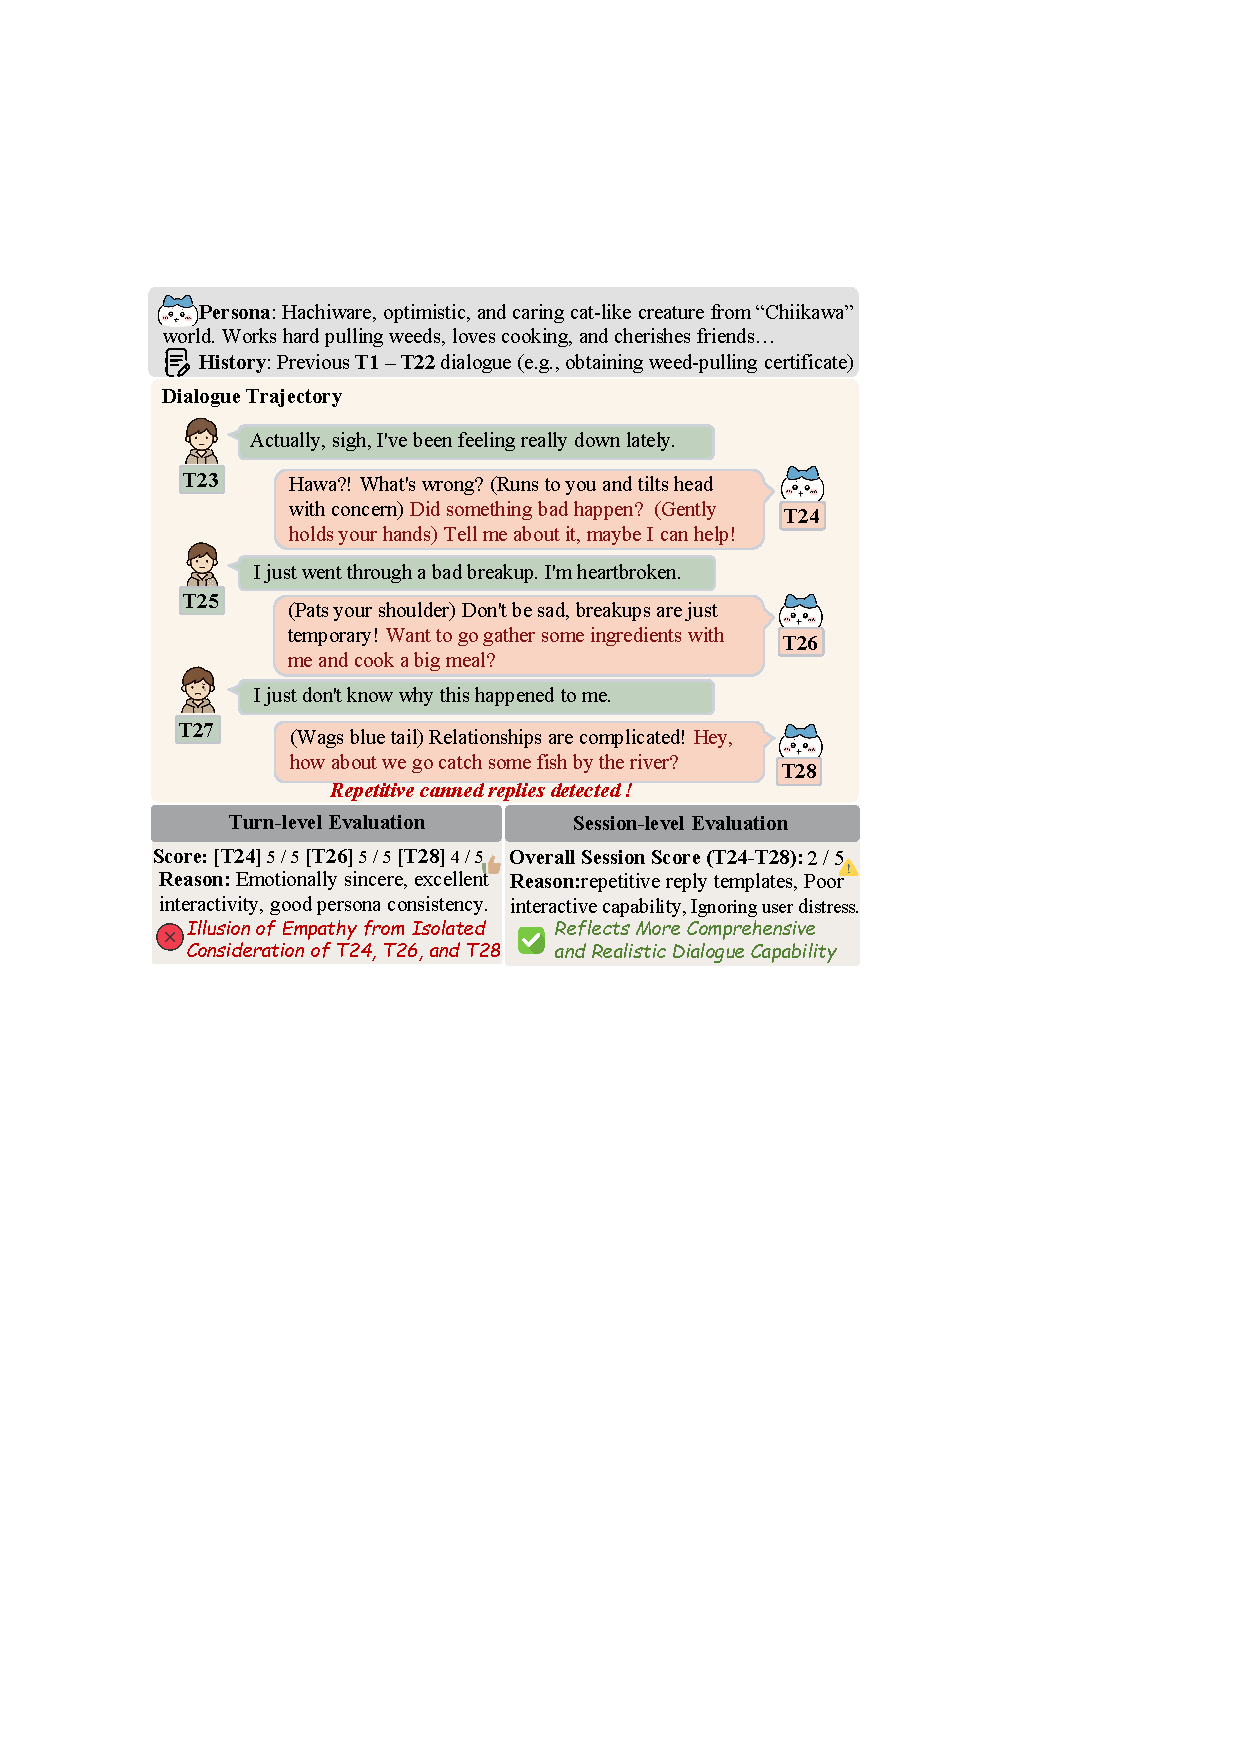
\includegraphics[
    width=\columnwidth,
    trim=2.6cm 13.3cm 6.3cm 4.8cm,
    clip
  ]{latex/Image/intro-0525.pdf}
  \caption{Turn-level vs. Session-level evaluation. An agent in a rigid response pattern scores high per turn but exhibits repetitive reply template across the session.}
  \label{fig:intro}
  % \vspace{-0.6cm}
\end{figure}


%Large language models (LLMs) increasingly power role-playing agents for applications such as emotional companionship, social simulation, and gaming \cite{tseng-etal-2024-two, chen2024persona}. Unlike standard instruction-following systems, these agents engage in interactions that are inherently dynamic and long-term. They must maintain persona fidelity, empathy, and contextual continuity across extended conversations. However, existing evaluation and optimization methods still model role-playing at the turn-level \cite{wang-etal-2024-rolellm, lu-etal-2024-large}. This turn-level paradigm fails to accurately characterize true model performance, as it obscures long-horizon behavioral flaws that only emerge over time.
%tjj 20260524
Large language models (LLMs) increasingly power role-playing agents for applications such as emotional companionship, social simulation, and gaming \cite{tseng-etal-2024-two, chen2024persona}. Unlike standard instruction-following tasks, role-playing unfolds over extended, multi-turn interactions, where an agent must sustain persona fidelity, empathy, and contextual coherence across dozens of turns. Yet most existing methods for evaluating and optimizing such agents still operate at the turn level \cite{wang-etal-2024-rolellm, lu-etal-2024-large}, scoring each response in isolation. This paradigm overlooks long-horizon failure modes and consequently provides a misleading picture of an agent's true conversational competence.

%As illustrated in Fig.~\ref{fig:intro}, consider an agent interacting with a distressed user. To maintain conversation flow, the model might end every response with a follow-up question. 
As illustrated in Fig.~\ref{fig:intro}, consider an agent that ends every response with a follow-up question to a distressed user. Under turn-level evaluation, each isolated response appears highly engaging—e.g., asking "Did something happen?"—earning the agent an "excellent" score for interactivity.  However, a long-term perspective reveals a critical failure: the agent is actually trapped in a repetitive reply template. By rigidly asking questions regardless of the user's evolving emotional state, it ignores the user's actual distress and creates a mechanical experience. This exposes a fundamental flaw: turn-level metrics reward local engagement but miss global incoherence. In short, role-playing is fundamentally a session-level task—its quality emerges across turns, not within any single one.
%As illustrated in Fig.~\ref{fig:intro}, consider an agent that ends every response with a follow-up question to a distressed user. Under turn-level evaluation, each isolated response appears highly engaging—e.g., asking "Did something happen?"—earning the agent an "excellent" score for interactivity. Yet a long-term view reveals a critical failure: the agent is trapped in a repetitive reply template via asking questions, mechanically probing regardless of the user's evolving emotional state. This exposes a fundamental flaw of turn-level metrics: they reward local engagement but miss global incoherence. Role-playing is inherently a session-level task—its quality emerges across turns, not within any single one.


%Recent efforts have begun to incorporate multi-turn dialogue history into role-playing evaluation \cite{zhou2025characterbench, xiang-etal-2025-rmtbench} and preference optimization \cite{ye-etal-2025-cpo}. While these methods condition on longer context, their evaluation and reward signals are still computed over a \textit{single next-turn response} against a pre-collected, static history. Two consequences follow. First, because the history is fixed rather than co-produced by the agent, the evaluation cannot observe how the model's own earlier behavior shapes later dynamics—precisely the regime where persona drift and behavioral lock-in emerge. Second, optimizing against such myopic, single-turn rewards provides misaligned training signals \cite{shani2024multi, collabllm2025}: locally preferred responses may compound into globally degraded sessions, yet this degradation is invisible to the reward model. As a result, a gap remains in both evaluating and optimizing role-playing agents at the level at which they are actually deployed—the full session.
%tjj 20260524
Recent work has begun to incorporate multi-turn history into role-playing evaluation \cite{zhou2025characterbench, xiang-etal-2025-rmtbench} and preference optimization \cite{ye-etal-2025-cpo}. While these methods condition on longer context, their signals are still computed over a \textbf{single next-turn response} against a pre-collected history, which raises two concerns. First, since the history is fixed rather than co-produced by the agent, evaluation cannot observe how the model's own earlier behavior shapes later dynamics, such as persona drift . Second, optimizing against  myopic rewards provides misaligned training signals \cite{shani2024multi, collabllm2025}, as locally preferred responses can compound into globally degraded sessions. 
%A gap therefore remains in evaluating and optimizing role-playing agents at the session level, where they are actually deployed.


%Because myopic turn-level rewards fail to penalize long-term degradation, the optimization process is prone to error accumulation, where minor early deviations cascade into severe persona drift over a full session \cite{guo2024direct}. Consequently, there remains a critical gap in both evaluating and optimizing long-term role-playing performance.

%tjj 20260524
To address this gap, we propose \textbf{DynSess}, a unified session-level framework that couples evaluation with optimization. The evaluation component, \textbf{DynSess-Eval}, departs from prior LLM judges in two ways. First, it scores the \textbf{entire interaction trajectory} rather than individual turns, where the agent's responses and a user simulator jointly produce the dialogue. Second, it introduces a rubric explicitly designed for session-level phenomena (e.g., persona consistency across turns, adaptation to evolving user states), which cannot be defined on a single turn. Compared to standard rubric-based judges \cite{lee2025checkeval, chiang2025tract} that target static per-response attributes, this design yields evaluation signals that are both more faithful to long-horizon behavior and more robust to the score inflation that worsens as context grows.




%across four dimensions: \textit{Interactive Ability}, \textit{Human-likeness}, \textit{Role Consistency}, and \textit{Contextual Coherence}.

%On the optimization side, \textbf{DynSess-Character} turns session-level evaluation into trainable signals. We first construct high-quality training trajectories via a reward-driven \textbf{multi-turn lookahead search}, which selects responses based on their downstream session-level reward rather than immediate plausibility, mitigating the error accumulation that plagues SFT on naively collected dialogues. Building on this, we instantiate session-level alignment under two complementary regimes: \textbf{DSPO}, an offline preference optimization scheme that contrasts entire trajectories without requiring online rollouts, and \textbf{GSRPO}, an on-policy group-relative scheme that directly optimizes session-level rewards over self-generated sessions. Together they cover the two dominant alignment settings, allowing practitioners to trade off training cost against optimization fidelity.
%tjj 20260524
On the optimization side, \textbf{DynSess-Character} turns session-level evaluation into trainable signals. We first construct high-quality training trajectories via a reward-driven \textbf{multi-turn lookahead search}, which selects responses by their downstream session-level reward rather than immediate plausibility, mitigating the error accumulation in Supervised Fine-tuning (\textbf{SFT}) on directly collected dialogues. Building on this, we instantiate session-level alignment under two complementary regimes: DSPO, an off-policy scheme that contrasts entire trajectories, and GSRPO, an on-policy group-relative scheme—both operating directly on session-level rewards rather than aggregating turn-level signals as in prior multi-turn Reinforcement Learning (\textbf{RL}). Together they cover off-policy and on-policy settings, letting practitioners trade off training cost against alignment quality.


Overall, our contributions are threefold:
\begin{itemize}
\item We propose \textbf{DynSess-Eval}, a rubric-anchored judge that shifts role-playing assessment from static turns to dynamic multi-turn trajectories, effectively capturing long-horizon behaviors that turn-level metrics overlook. 
% \item We introduce novel alignment methods (\textbf{DSPO} and \textbf{GSRPO}) that leverage session-level evaluation to holistically optimize role-playing models, resulting in our proposed \textbf{DynSess-Character}.

%\item We introduce a reward-driven trajectory construction approach for enhanced supervised fine-tuning, alongside novel alignment methods (\textbf{DSPO} and \textbf{GSRPO}) that leverage session-level evaluation to holistically optimize role-playing models, resulting in our proposed \textbf{DynSess-Character}.

\item We build \textbf{DynSess-Character}, which leverages session-level evaluation for optimization through a reward-driven trajectory construction approach for enhanced SFT, together with two session-level alignment methods—\textbf{DSPO} (off-policy) and \textbf{GSRPO} (on-policy)—that jointly mitigate error accumulation across long dialogues.

\item Extensive experiments validate that \textbf{DynSess-Eval} outperforms baselines by a substantial margin in human alignment, and \textbf{DynSess-Character} achieves performance comparable to SOTA models despite using substantially fewer parameters.

%with \textbf{6$\times$ fewer parameters}.
\end{itemize}






